% =============================================================
%  SECTION: Physical Property Analysis — Krypton g(r)
%  ASSIGNED TO: [Person Name]
%
%  REQUIRED CONTENT:
%   - Real-world parameters for Krypton (eps, sigma)
%   - g(r) plot scaled to Ångströms
%   - State identification (solid or liquid?) with physical justification
%   - Confirmation that g(r) → 1.0 at large r
%   - (Optional, if chosen) MSD vs time (ps), diffusion coefficient D
%
%  GUIDING QUESTIONS:
%   HOW do we convert from reduced units to real units?
%   WHAT does the peak structure of Kr g(r) tell us about nearest-neighbour distance?
%   HOW does the Kr g(r) compare to ideal FCC peak positions?
%   WHY do we confirm g(r)→1? What does it mean if it doesn't?
% =============================================================

\newpage
\section{Physical Property Analysis: Krypton}

\subsection{Krypton Parameters}

To convert simulation results from reduced units to real physical quantities, we use the Lennard-Jones parameters for Krypton from Table 5.1 of LeSar:

\begin{table}[H]
    \centering
    \caption{Lennard-Jones parameters for Krypton used in this work.}
    \label{tab:kr_params}
    \begin{tabular}{lcc}
        \toprule
        \textbf{Parameter} & \textbf{Symbol} & \textbf{Value} \\
        \midrule
        Well depth & $\eps$ & $0.0140$\,eV \\
        Well depth (thermal) & $\eps/k_B$ & $162.46$\,K \\
        Atomic diameter & $\sigma$ & $3.65$\,\AA \\
        \bottomrule
    \end{tabular}
\end{table}

The unit conversions used are:
\begin{align}
    r\,[\text{\AA}] &= r^* \times \sigma_{\text{Kr}} = r^* \times 3.65\,\text{\AA} \label{eq:r_conv}\\
    T\,[\text{K}]   &= \Tstar \times (\eps/k_B)_{\text{Kr}} = \Tstar \times 162.46\,\text{K} \label{eq:T_conv}
\end{align}

We ran simulations at two representative temperatures: $\Tstar = 0.4$ ($\approx 65$\,K, expected solid) and $\Tstar = 1.0$ ($\approx 162$\,K, expected liquid). Simulation parameters are given in Table~\ref{tab:params}.

\subsection{Radial Distribution Function: \texorpdfstring{$g(r)$}{g(r)}}

\begin{figure}[H]
    \centering
    \begin{subfigure}[b]{0.48\linewidth}
        \centering
        % \includegraphics[width=\linewidth]{figures/kr_gr_T04.pdf}
        \caption{$\Tstar = 0.4$ ($T \approx 65$\,K)}
        \label{fig:kr_gr_solid}
    \end{subfigure}
    \hfill
    \begin{subfigure}[b]{0.48\linewidth}
        \centering
        % 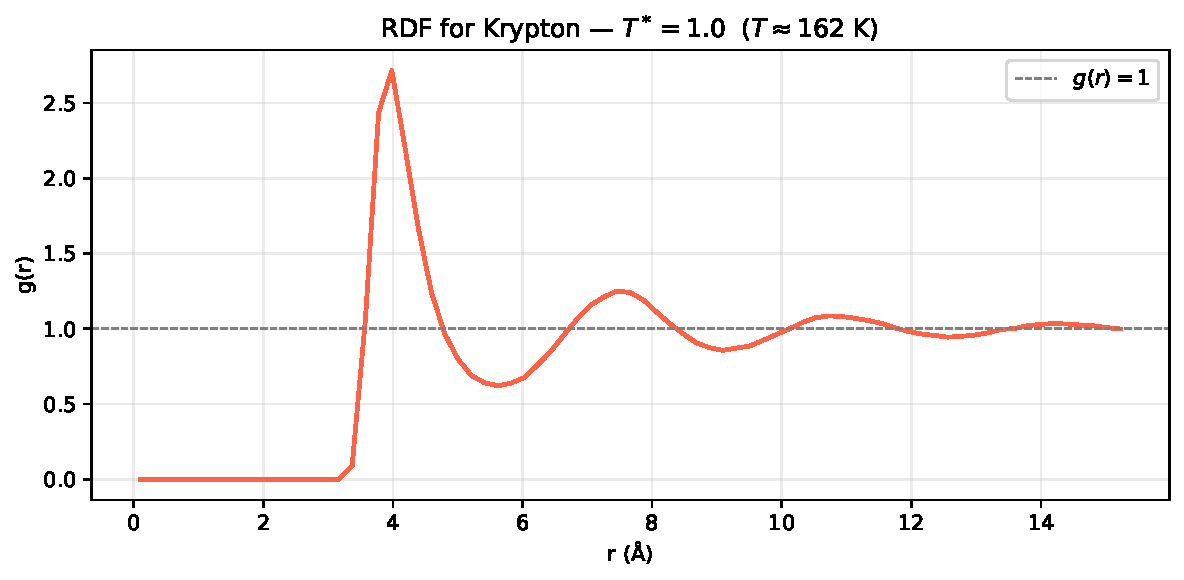
\includegraphics[width=\linewidth]{figures/kr_gr_T10.pdf}
        \caption{$\Tstar = 1.0$ ($T \approx 162$\,K)}
        \label{fig:kr_gr_liquid}
    \end{subfigure}
    \caption{Radial distribution function $g(r)$ of Krypton at two temperatures. The horizontal axis is scaled to real units using $\sigma_{\text{Kr}} = 3.65$\,\AA. The dashed line at $g(r) = 1$ is the ideal-gas asymptote.}
    \label{fig:kr_gr}
\end{figure}

% [INSERT ACTUAL PLOTS — provide these to the report writer]

\subsection{State Identification and Physical Interpretation}

% Explain the peak structure for each temperature:
%
% T* = 0.4 (SOLID):
%   - Sharp, distinct peaks at well-defined r values.
%   - Multiple coordination shells visible.
%   - Peak positions correspond to FCC neighbour distances.
%   - First peak near r* ≈ 1.12σ = ~4.1 Å.
%
% T* = 1.0 (LIQUID):
%   - Broad first peak, rapidly decaying oscillations.
%   - g(r) reaches 1.0 after ~3 peaks.
%   - No long-range order.

\subsubsection{Solid Phase ($\Tstar = 0.4$, $T \approx 65$\,K)}

% [WRITE INTERPRETATION HERE]

\subsubsection{Liquid Phase ($\Tstar = 1.0$, $T \approx 162$\,K)}

% [WRITE INTERPRETATION HERE]

\subsection{Normalization Check: \texorpdfstring{$g(r) \to 1$}{g(r)→1}}

% Confirm that g(r) asymptotes to 1.0 at large r in both cases.
% Report the value at the last bin.

At $r \approx L/2 = [value]$\,\AA, the measured $g(r) = [value]$ for $\Tstar = 0.4$ and $g(r) = [value]$ for $\Tstar = 1.0$, both within [tolerance] of the expected asymptote of 1.0.

% [WRITE DISCUSSION — what would it mean if g(r) didn't reach 1?]

% =============================================================
%  OPTIONAL SECTION — include only if MSD was chosen
% =============================================================
% \subsection{Mean Square Displacement and Diffusion Coefficient}
%
% (Include this section only if your group also computed MSD)
%
% \subsubsection{Unwrapped Coordinates}
% [EXPLAIN WHY UNWRAPPED IS NECESSARY]
%
% \subsubsection{MSD vs. Time}
% \begin{figure}[H]
%     \centering
%     % \includegraphics[width=0.75\linewidth]{figures/kr_msd.pdf}
%     \caption{MSD vs. time in picoseconds for Krypton at $\Tstar = 1.0$.}
% \end{figure}
%
% \subsubsection{Diffusion Coefficient}
% From the Einstein relation $D = \lim_{t\to\infty} \frac{1}{6t}\langle R^2(t) \rangle$,
% the slope of the linear regime gives:
% \begin{equation}
%     D_{\text{Kr}} = [value]\,\text{m}^2/\text{s}
% \end{equation}
